% MODELO CONEM 2016
\documentclass[10pt,fleqn,a4paper]{article}
\usepackage{abcm}
\usepackage{float}

\begin{document}
    
    % CABEÇALHO
    \fancypagestyle{firststyle}
	{
   		\lhead{\emph{Anais do XXIV Encontro de Iniciação Científica e Pós-Graduação do ITA - XXIV ENCITA / 2018
	Instituto Tecnológico de Aeronáutica, São José dos Campos, SP, Brasil, XXIV 18 de outubro de 2018}}  
	}
    \thispagestyle{firststyle}
    \vspace{-.5cm}
    \hspace{-.8cm}
    \begin{tabular}{p{\textwidth}}
    \begin{center}
    \vspace{-.6cm}
    \title{Controle para Rastreio de Trajetória por um Robô com Acionamento Diferencial Utilizando Retroalimentação por Câmera}
    \end{center}
    \textbf{Igor Mourão Ribeiro}\\
    \small{Instituto Tecnológico de Aeronáutica}\\
    \small{Rua H8C, 317, CTA}\\
    \small{12.228-462 - São José dos Campos/SP}\\
    \small{Bolsista PIBIC - CNPq}\\
    \small{igormr98mr@gmail.com}\\
    \\ 
    \textbf{Paulo Marcelo Tasinaffo}\\
    \small{Instituto Tecnológico de Aeronáutica}\\
    \small{Divisão de Ciência da Computação}\\
    \small{Praça Marechal Eduardo Gomes, 50}\\
    \small{12.229-900 – São José dos Campos / SP}\\
    \small{tasinaffo@ita.br}\\
    \\ 
    \textbf{Marcos Ricardo Omena de Albuquerque Máximo}\\
    \small{Instituto Tecnológico de Aeronáutica}\\
    \small{Divisão de Ciência da Computação}\\
    \small{Praça Marechal Eduardo Gomes, 50}\\
    \small{12.229-900 – São José dos Campos / SP}\\
    \small{maximo.marcos@gmail.com}\\
    \\
    \abstract{\textbf{Resumo:} Devido à alta complexidade existente nos algoritmos de funcionamento de um robô humanoide, é fundamental possuir ferramentas de interface com o usuário para o desenvolvimento do sistema. Estas ferramentas possuem a finalidade de fornecer uma visualização dos algoritmos envolvidos de forma clara para o usuário. Após uma fase de pesquisa, foi decidido utilizar o framework rqt, uma plataforma baseada em Qt que permite o desenvolvimento de interfaces gráficas para ROS (Robot Operational System), assim possibilitando criar um sistema de telemetria para o robô. Com este intuito, foram desenvolvidas três ferramentas iniciais. A primeira, feita antes da pesquisa sobre o framework rqt, foi escrita utilizando apenas a plataforma Qt. Ela é uma interface que permite anotar imagens e gerar tabelas de cores utilizando as funções de treinamento de redes neurais presentes no software MATLAB. A segunda utiliza o framework rqt e é uma ferramenta de teste e calibração do algoritmo de visão computacional do robô humanoide. A última ferramenta é um controle remoto do robô que permite variar a sua velocidade para facilitar a depuração do código.}\\
    \keywords{\textbf{Palavras-chave:} robótica, estratégia, tomada de decisão}\\
    \end{tabular}
    
no max 4000 caracteres no resumo
artigo de no máx 10 páginas
tamanho máximo do pdf: 2,5 MB
    \section{INTRODUÇÃO}
        
	A ITAndroids é uma equipe de alunos do ITA, supervisionada por um professor, que participa de diversas competições de robótica nacionais e internacionais. Uma das categorias em que a ITAndroids participa é a do robô humanoide, que consiste em desenvolver um time de robôs capazes de jogar futebol. Esta tarefa envolve uma série de desafios complexos que variam desde a construção do robô até a sua tomada de decisões.  
	
	Neste contexto, é fundamental a presença de algoritmos robustos para a realização das diversas ações do robô, tornando essenciais as ferramentas de testes, calibração e depuração. Equipes reconhecidas no cenário internacional, como a B-Human e a Nimbro-OP, possuem várias ferramentas com este intuito, como são apresentadas em Roffer et al. (2013) e em Allgeuer et al. (2013).

	Essas ferramentas devem possibilitar o teste dos algoritmos em tempo real, criando um sistema de telemetria com o robô. Além disso, é interessante que elas também possibilitem testes sem a presença do robô, assim facilitando a depuração e calibração do código.


    \section{RESULTADOS OBTIDOS}
        
	Os resultados a seguir foram obtidos estudando o comportamentos de equipes adversárias na competição, além de diversos testes com o time de robôs da ITAndroids contra si mesmo em simulações computacionais em um simulador feito pela própria equipe, como mostrado na Figura \ref{fig:simulator}.

\begin{figure}[H]
	\centering
	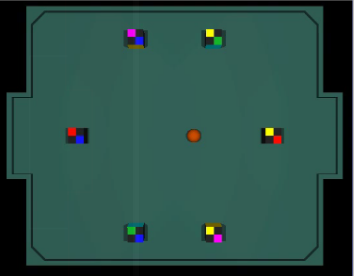
\includegraphics[width=0.6\textwidth]{figures/SimulatorWithoutButtons.png}
	\caption{Simulador da ITAndroids.}
	\label{fig:simulator}
\end{figure}

\subsection{Goleiro}

A BT criada para o goleiro está representada na Figura \ref{fig:goalier_bt}.

\begin{figure}[H]
	\centering
	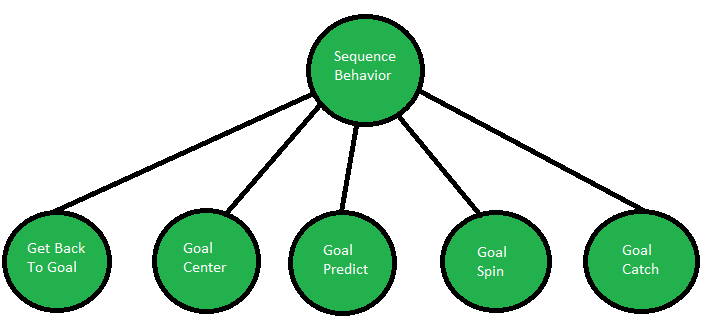
\includegraphics[width=0.8\textwidth]{figures/Goalier_BT.png}
   	\caption{Behavior Tree para o goleiro.} \label{fig:goalier_bt}
\end{figure}

Como visto, ela é composta por um nó do tipo Sequence Behavior, que irá executar os seus filhos em sequência. Esse papel, então, executa as seguintes ações prioritando as primeiras a aparecerem na seguinte lista:

\begin{itemize}

\item \textbf{Get Back to Goal Behavior} Volta para o gol, caso que, se por algum motivo ele esteja fora do próprio.

\item \textbf{Goal Center} Fica centralizado no gol quando a bola estiver longe, de forma que o jogador possa rapidamente ir para qualquer um dos lados quando a bola se aproximar.

\item \textbf{Goal Predict} Prediz para onde a bola irá quando ela estiver rápida e longe do gol.

\item \textbf{Goal Spin} Gira quando está perto da bola e não tem oponente perto da bola para jogá-la para longe.

\item \textbf{Goal Catch} Comportamento que o goleiro deverá fazer quando não fizer nenhum outro, por isso sua última posição na sequência. Ele acompanha o movimento da bola com o goleiro sobre a linha do gol.

\end{itemize}



\subsection{Principal}

Já para o principal, a árvore \ref{fig:principal_bt} foi desenvolvida, sendo a árvore mais complexa dentre os papéis.

\begin{figure}[H]
	\centering
	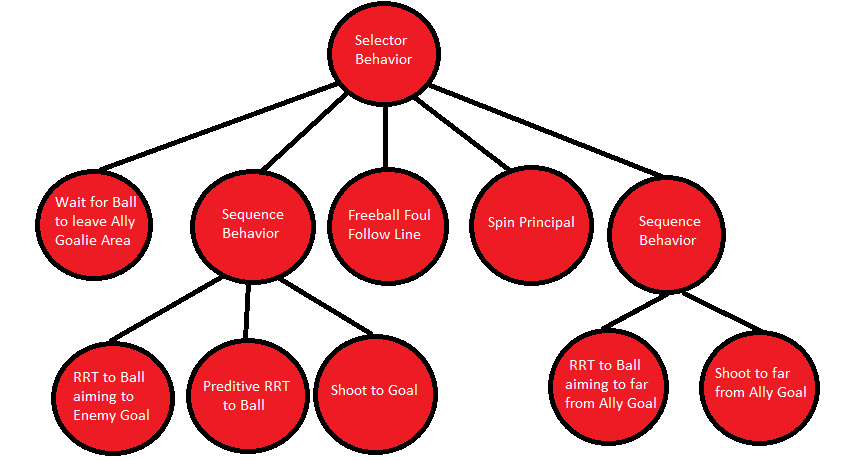
\includegraphics[width=0.8\textwidth]{figures/Principal_BT.png}
   	\caption{Behavior Tree para o principal.} \label{fig:principal_bt}
\end{figure}   

Conforme a Figura \ref{fig:principal_bt}, a raiz da árvore do principal é um Selector Behavior que escolhe uma das ações a ser realizada. Essa BT tem mais dois outros nós compostos, que são dois Sequence Behavior usados para o posicionamento atrás da bola, seguido pelo chute. Uma descrição dos nós folha utilizados se encontra abaixo:

\begin{itemize}

\item \textbf{Wait for Ball to leave Ally Goalie Area} Esse Behavior utiliza a Triangução de Delaunay, com a mesma interface desenvolvida na Figura \ref{fig:delaunay_interface}. Esse comportamento deve evitar que o jogador entre na área do goleiro para não sofrer penâlti, conforme descrito na Figura \ref{fig:penalty}. O jogador se pocionará de acordo com posições escolhidas pelo usuário, calibradas com o arquivo de configuração do mesmo modelo da Figura \ref{fig:text_config_delaunay}.

\item \textbf{RRT to Ball aiming to Enemy Goal} Irá usar o algoritmo de planejamento de trajetórias RRT para se deslocar atrás da bola com direção apontando para o gol oponente. Usado para se aproximar da bola e, em seguida, trocar para o próximo behavior, o Predictive RRT to Ball.

\item \textbf{Predictive RRT to Ball} Usa uma predição linear considerando que a bola continuará na mesma velocidade. Usado para se chegar na bola com mais precisão quando próximo a ela. Chega atrás da bola mirando para o gol.

\item \textbf{Shoot to Goal} Esse behavior só é chamado quando o jogador já está alinhado com a bola e o gol oponente. Esse comportamento acelera rapidamente o robô em linha reta para chegar no gol com uma velocidade alta.

\item \textbf{Free Ball Foul Follow Line} Esse behavior é um específico para situações de falta do tipo Bola Livre, conforme descrito em \ref{fig:bola_livre}. Quando for detectado uma dessas posições, o jogador deve acelerar o mais rápio possível em direção à bola para ter o controle dela antes do oponente.

\item \textbf{Spin Principal} Esse nó deve ser chamado quando a bola estiver em um dos quatros campos do campo. Caso seja um campo defensivo, o jogador irá girar para jogar a bola para frente; caso seja um na zona de ataque, o jogador girará para por a bola no centro do campo e continuar o ataque.

\item \textbf{RRT to Ball aiming to far from Ally Goal} Irá usar o algoritmo de planejamento de trajetórias RRT para se deslocar atrás da bola com direção apontando para a zona de ataque (longe do gol aliado). Usado para se aproximar da bola e se posicionar para, em seguida, chamar o Behavior Shoot to Far from Ally Goal.

\item \textbf{Shoot to Far from Ally Goal} Esse behavior só é chamado quando o jogador já está alinhado com a bola e o para frente (para longe do gol alidado). Esse comportamento acelera rapidamente o robô em linha reta para por a bola na zona de ataque.

\end{itemize}


\subsection{Auxiliar}

O auxiliar, por sua vez, tem uma Behavior Tree muito simples, representada por apenas um nó que tem como função se posicionar em lugar ótimo com Triangulação de Delaunay\cite{delaunay34}. Sua árvore, é representada simplesmente pela Figura \ref{fig:auxiliar_bt}.

\begin{figure}[H]
	\centering
	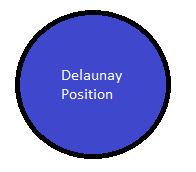
\includegraphics[width=0.4\textwidth]{figures/Auxiliar_BT.png}
   \caption{Behavior Tree para o auxiliar.} \label{fig:auxiliar_bt}
\end{figure}

	\section{CONCLUSÕES}
	
	O projeto de Iniciação Científica apresentou bons resultados, especialmente quanto à vitória da equipe do ITA até às quartas de final da CBR 2017, rendendo o sétimo lugar à equipe dentre mais de 25 equipes participantes. Além do fato de que a ITAndroids conquistou o primeiro lugar na competição nacional de VSSS Copa Turing 2017, que ocorreu no final de setembro de 2017.

	Do ponto de vista técnico, o uso do algoritmo da Behavior Tree, já consagrado e usado por times de nível mundial, se mostrou factível e funcional em partidas reais de competições. Contudo, problemas como pouca escalabilidade e pouca reutilizabilidade se mostraram presentes na estratégia desenvolvida. Isso significa que mudanças ainda deverão ser feitas nas BT, principalmente a respeito do uso de mais nós do tipo paralelo para remover esses problemas citados.

    \section{AGRADECIMENTOS}
    
	Agradeço ao CNPq, pelo apoio financeiro e motivacional.
	
	Agradeço à ITAndroids, equipe que representa o ITA na competição da LARC/CBR, pela ideia do projeto, pela disponibilidade do robô real para implementação e oportunidade de aplicação dos métodos estudados.

	Agradeço ao professor doutor Paulo Marcelo Tasinaffo, meu orientador, e ao professor doutor Marcos Ricardo de Omena Máximo, co-orientador, ambos da Divisão da Ciência da Computação do ITA, pelo apoio nos estudos e no desenvolvimento do projeto.

    % REFERÊNCIAS
    \section{REFERÊNCIAS}
        \bibliographystyle{abcm}
        \bibliography{bibliografia}

    \section{RESPONSABILIDADE AUTORAIS}

        Os trabalhos escritos em português ou espanhol devem incluir (após direitos autorais) título, os nomes dos autores e afiliações, o resumo e as palavras chave, traduzidos para o inglês e a declaração a seguir, devidamente adaptada para o número de autores.
    
        O(s) autor(es) é(são) o(s) único(s) responsável(is) pelo conteúdo deste trabalho.

% % RESUMO EM INGLES
%
%\noindent{
%   \\ 
%    \begin{tabular}{||p{\textwidth}}
%    \begin{center}
%    \vspace{-.6cm}
%    \title{AFTER FULL PAPER IN PORTUGUESE OR SPANISH, IT’S NECESSARY THE ABSTRACT IN ENGLISH}
%    \end{center}
%    \authors{First Author’s Name, e-mail1$^1$} \\
%    \authors{Second Author’s Name, e-mail$^2$} \\
%    \authors{Third Author’s Name, e-mail$^2$} \\\\
%    \institution{$^1$Institution and address for first author} \\
%    \institution{$^2$Institution and address for second and third authors} \\
%    \\
%    \authors{\textcolor[rgb]{0.98,0.00,0.00}{Same format for other authors and institutions, if any.}} \\
%    \\
%    \abstract{\textbf{Resumo:} The purpose of these instructions is to serve as a guide for formatting papers to be published in the Proceedings of the IX CONEM.  The abstract should describe the objectives, the methodology and the main conclusions of the paper in less than 4000 characters in a single paragraph.  It should not contain either formulae or bibliographic references. The full paper will be published in the proceedings of the event.}\\
%    \keywords{\textbf{Palavras-chave:} keyword 1, keyword 2, keyword 3 (up to 5 keywords) }\\
%    \end{tabular}
%}

\end{document}